\section{Durchführung}
\subsection{Aufbau}
Für den Versuch wurde der Aufbau aus der Abbildung verwendet. Die Brückenschaltung wurde von einem Sinusgenerator gespeist und die Brückenspannung von einem Selektivverstärker gefiltert. Das Ausgangssignal wurde auf einem Voltmeter angezeigt.
\subsection{Messung der Filterkurve}
Zur Messung der Filterkurve wurde die Frequenz des Sinusgenerators in einem Bereich zwischen $20$ und $40 kHz$ bei einer festen Filterfrequenz variirt und die Ausgangsspannung gemessen.
\subsection{Messung der Suszeptibilität}
Im Zuge der Suszeptibilitätsmessung wurde zunächst die Brücke ohne Probe abgeglichen und der eingestellte Widerstand
sowie die verbleibende Restspannung gemessen wurde. Anschließend wurde die Probe in die Spule eingeführt und die resultierende Brückenspannung gemessen. Schließlich wurde die Brücke erneut abgeglichen und die Restspannung sowie der neue Widerstandswert notiert. Weiterhin wurde mithilfe einer Schieblehre Länge und Durchmesser der Probe bestimmt. Dieser Prozess wurde für eine weitere Probe wiederholt.
\begin{figure}[h]
    \label{fig:block}
    \centering
    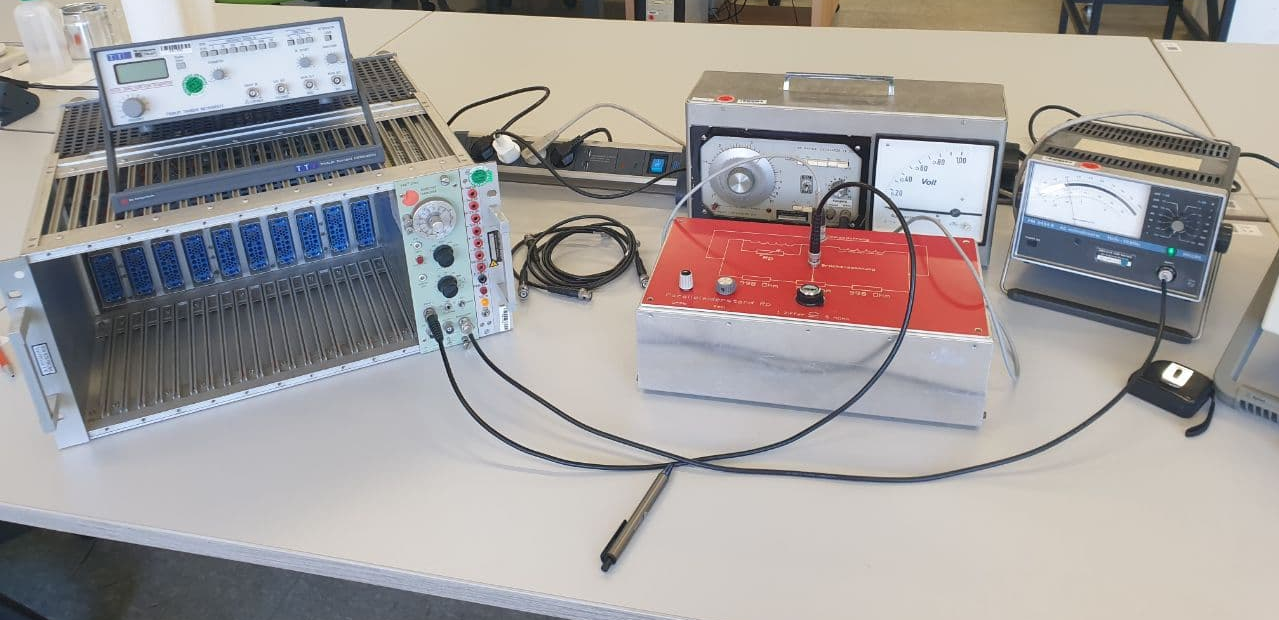
\includegraphics[width=10cm]{Aufbau.png}
    \caption{Versuchsaufbau}
\end{figure}
